\documentclass[conference]{IEEEtran}
% \documentclass[conference]{acmart}
\usepackage[utf8]{inputenc}
\usepackage[italian]{babel}
\usepackage{graphicx}
\usepackage{adjustbox}
\usepackage{xargs}
\usepackage{amsmath}
\usepackage{amssymb}
\usepackage{booktabs}
\usepackage{listings}
\usepackage{xcolor}
\usepackage{hyperref}
\hypersetup{hypertexnames=false}
\usepackage{cite} % IEEE specific package for bibliography management
\usepackage{tabularx}
\usepackage{float}

% Configurazione
\definecolor{codegreen}{rgb}{0,0.6,0}
\definecolor{codegray}{rgb}{0.5,0.5,0.5}
\definecolor{codepurple}{rgb}{0.58,0,0.82}
\definecolor{backcolour}{rgb}{0.95,0.95,0.92}

\lstdefinestyle{mystyle}{
    backgroundcolor=\color{backcolour},   
    commentstyle=\color{codegreen},
    keywordstyle=\color{magenta},
    numberstyle=\tiny\color{codegray},
    stringstyle=\color{codepurple},
    basicstyle=\ttfamily\footnotesize,
    breakatwhitespace=false,         
    breaklines=true,                 
    captionpos=b,                    
    keepspaces=true,                 
    numbers=left,                    
    numbersep=5pt,                  
    showspaces=false,                
    showstringspaces=false,
    showtabs=false,                  
    tabsize=2
}
\lstset{style=mystyle}

% ACM Configuration
%\setcopyright{none}
%\acmConference[SABD 2025/26]{Sistemi e Architetture per Big Data}{Giugno 2026}{Roma, Italia}
%\acmDOI{}
%\acmISBN{}


% Page numbering
\makeatletter
\def\ps@headings{%
\def\@oddhead{\mbox{}\scriptsize\rightmark \hfil \thepage}%
\def\@evenhead{\scriptsize\thepage \hfil \leftmark\mbox{}}%
\def\@oddfoot{}%
\def\@evenfoot{}}
\makeatother

% \throughputChart[width]{nome_file}{caption}{label}
\newcommandx{\throughputChart}[4][1=0.95\linewidth]{%
    \begin{figure}[H]
        \centering
        % trim={<sinistra> <basso> <destra> <alto>}
        \adjustbox{trim={0.01\width} {0.805\height} {0.00\width} {0.04\height}, clip}{%
            \includegraphics[width=#1]{../Results/charts/#2}%
        }
        \caption{#3}
        \label{#4}
    \end{figure}%
}

% \latencyChart[width]{nome_file}{caption}{label}
\newcommandx{\latencyChart}[4][1=0.99\linewidth]{%
    \begin{figure}[H]
        \centering
        \adjustbox{trim={0.01\width} {0.455\height} {0.00\width} {0.308\height}, clip}{%
            \includegraphics[width=#1]{../Results/charts/#2}%
        }
        \caption{#3}
        \label{#4}
    \end{figure}%
}

% \checkpointChart[width]{nome_file}{caption}{label}
\newcommandx{\checkpointChart}[4][1=0.95\linewidth]{%
    \begin{figure}[H]
        \centering
        \adjustbox{trim={0.01\width} {0.348\height} {0.00\width} {0.55\height}, clip}{%
            \includegraphics[width=#1]{../Results/charts/#2}%
        }
        \caption{#3}
        \label{#4}
    \end{figure}%
}

% \outoforderChart[width]{nome_file}{caption}{label}
\newcommandx{\outoforderChart}[4][1=0.85\linewidth]{%
    \begin{figure}[H]
        \centering
        \adjustbox{trim={0.01\width} {0.01\height} {0.00\width} {0.650\height}, clip}{%
            \includegraphics[width=#1]{../Results/charts/#2}%
        }
        \caption{#3}
        \label{#4}
    \end{figure}%
}

% \nodeChart[width]{nome_file}{caption}{label}
\newcommandx{\nodeChart}[4][1=0.95\linewidth]{%
    \begin{figure}[H]
        \centering
        \adjustbox{trim={0.01\width} {0.31\height} {0.00\width} {0.08\height}, clip}{%
            \includegraphics[width=#1]{../Results/charts/#2}%
        }
        \caption{#3}
        \label{#4}
    \end{figure}%
}

\newcommandx{\queryOneChart}[4][1=0.90\linewidth]{%
    \begin{figure}[H]
        \centering
        \adjustbox{trim={0.00\width} {0.44\height} {0.00\width} {0.072\height}, clip}{%
            \includegraphics[width=#1]{../Results/plots/#2}%
        }
        \caption{#3}
        \label{#4}
    \end{figure}%
}

\newcommandx{\queryTwoOneHourChart}[4][1=0.95\linewidth]{%
    \begin{figure}[H]\centering
        \adjustbox{trim={0.00\width} {0.67\height} {0.00\width} {0.078\height}, clip}{\includegraphics[width=#1]{../Results/plots/#2}}
        \caption{#3}
        \label{#4}
    \end{figure}%
}

\newcommandx{\queryTwoSixHourChart}[4][1=0.95\linewidth]{%
    \begin{figure}[H]\centering
        \adjustbox{trim={0.00\width} {0.415\height} {0.00\width} {0.33\height}, clip}{\includegraphics[width=#1]{../Results/plots/#2}}
        \caption{#3}
        \label{#4}
    \end{figure}%
}

\newcommandx{\queryTwoGlobalChart}[4][1=0.95\linewidth]{%
    \begin{figure}[H]\centering
        \adjustbox{trim={0.00\width} {0.16\height} {0.00\width} {0.58\height}, clip}{\includegraphics[width=#1]{../Results/plots/#2}}
        \caption{#3}
        \label{#4}
    \end{figure}%
}

\newcommandx{\queryThreeOneDayChart}[4][1=0.98\linewidth]{%
    \begin{figure}[H]\centering
        \adjustbox{trim={0.01\width} {0.64\height} {0.01\width} {0.05\height}, clip}{\includegraphics[width=#1]{../Results/plots/#2}}
        \caption{#3}
        \label{#4}
    \end{figure}%
}

\newcommandx{\queryThreeSevenDayChart}[4][1=0.98\linewidth]{%
    \begin{figure}[H]\centering
        \adjustbox{trim={0.01\width} {0.33\height} {0.01\width} {0.36\height}, clip}{\includegraphics[width=#1]{../Results/plots/#2}}
        \caption{#3}
        \label{#4}
    \end{figure}%
}

\newcommandx{\queryThreeGlobalChart}[4][1=0.98\linewidth]{%
    \begin{figure}[H]\centering
        \adjustbox{trim={0.01\width} {0.02\height} {0.01\width} {0.67\height}, clip}{\includegraphics[width=#1]{../Results/plots/#2}}
        \caption{#3}
        \label{#4}
    \end{figure}%
}


\pagestyle{headings}


\begin{document}

\title{Sky Analytics Stream \\ \vspace{0.15cm} \large Architettura Distribuita per l'Analisi in Tempo Reale del Traffico Aereo}

% IEEE Configuration
\author{
    \IEEEauthorblockN{Flavio Simonelli}
    \IEEEauthorblockA{Matricola 0365333\\
    Dipartimento di Ingegneria\\
    Università di Roma "Tor Vergata"\\
    flavio.simonelli@alumni.uniroma2.eu}
    \and
    \IEEEauthorblockN{Francesco Masci}
    \IEEEauthorblockA{Matricola 0365258\\
    Dipartimento di Ingegneria\\
    Università di Roma "Tor Vergata"\\
    francesco.masci.02@alumni.uniroma2.eu}
}

% ACM Configuration
% \author{Flavio Simonelli}
% \affiliation{%
%     \institution{Università di Roma "Tor Vergata"}
%     \city{Roma}
%     \country{Italia}
% }
% \email{flavio.simonelli@alumni.uniroma2.eu}
%
% \author{Francesco Masci}
% \affiliation{%
%     \institution{Università di Roma "Tor Vergata"}
%     \city{Roma}
%     \country{Italia}
% }
% \email{francesco.masci.02@alumni.uniroma2.eu}

% IEEE Configuration
\maketitle
\thispagestyle{headings}

% ------------------------------

\begin{abstract}
Questo lavoro presenta \textit{Sky Analytics Stream}, un'architettura distribuita per l'analisi e il monitoraggio in tempo reale del traffico aereo basata su Apache Flink e Apache Kafka. Il sistema riceve i dati da un simulatore ad alte prestazioni sviluppato in Go, in grado di riprodurre flussi di eventi storici in event-time con disordine controllato e fattori di accelerazione variabili. Attraverso un'unica topologia a grafo diretto aciclico, la pipeline esegue in parallelo tre analisi: aggregazioni orarie delle performance delle compagnie aeree, classifiche in tempo reale degli aeroporti con ritardi severi e stima dei percentili dei ritardi tramite l'algoritmo DDSketch. Risultati e metriche di telemetria sono storicizzati in InfluxDB e visualizzati tramite Grafana. La tolleranza ai guasti è garantita da checkpointing \emph{exactly-once} con stato incrementale gestito da RocksDB. La valutazione sperimentale analizza le prestazioni del sistema al variare del parallelismo, del disordine degli eventi e della frequenza dei checkpoint.
\end{abstract}

% ------------------------------

% IEEE Configuration
\begin{IEEEkeywords}
Apache Flink, Stream Processing, Apache Kafka, Traffico Aereo, Percentili Approssimati, Tolleranza ai Guasti, DDSketch, checkpointing.
\end{IEEEkeywords}

% ACM Configuration
% \keywords{}

% ------------------------------

% ACM Configuration
% \maketitle
% \thispagestyle{headings}

\section{Introduzione}\label{sec:introduction}

L'analisi tempestiva del traffico aereo richiede di elaborare flussi continui di dati per aggiornare metriche prestazionali e classifiche di ritardo in tempo reale. In questo contesto, l'accuratezza e la freschezza dei risultati dipendono dalla capacità di gestire le sfide intrinseche dello stream processing. In particolare, ritardi di rete, colli di bottiglia nell'ingestione e arrivi fuori ordine fanno sì che il tempo logico in cui un volo si verifica, ovvero l'\emph{event-time}, non venga rispettato nell'ordine di come gli eventi arrivano ai processori di elaborazione. Per fornire risultati coerenti e completi, è dunque cruciale definire politiche di watermarking e di gestione dei dati tardivi che bilancino correttamente la latenza e l'accuratezza delle aggregazioni.

Per affrontare tali sfide, questo lavoro presenta il progetto e la valutazione sperimentale di \textit{Sky Analytics Stream}, un'architettura distribuita progettata per elaborare un dataset storico di voli negli Stati Uniti (relativi al periodo gennaio--aprile 2025). Il dataset viene riprodotto in modo controllato tramite un simulatore ad alte prestazioni sviluppato in Go, in grado di iniettare dati in Apache Kafka applicando fattori di compressione temporale e introducendo disordine artificiale. La pipeline di elaborazione principale è realizzata in Apache Flink e implementa un singolo grafo aciclico ottimizzato per eseguire in parallelo tre analisi distinte:
\begin{enumerate}
    \item Il calcolo orario delle statistiche di volo per ciascuna compagnia aerea;
    \item Il tracciamento dinamico delle classifiche Top-10 degli aeroporti con i maggiori ritardi accumulati;
    \item La stima continua dei percentili dei ritardi.
\end{enumerate}

Il resto della relazione è organizzato come segue: la Sezione~\ref{sec:system_architecture} descrive l'architettura generale del sistema e il flusso dei dati; la Sezione~\ref{sec:implementation_details} approfondisce i dettagli implementativi delle singole componenti; la Sezione~\ref{sec:deployment_infrastructure} illustra l'infrastruttura di deployment; la Sezione~\ref{sec:experimental_evaluation} presenta la valutazione sperimentale e i risultati dei test prestazionali; infine, la Sezione~\ref{sec:conclusions_future_work} conclude il report delineando possibili sviluppi futuri.

% ------------------------------

\section{Architettura del Sistema}\label{sec:system_architecture}

L'architettura di \textit{Sky Analytics Stream} è concepita come una pipeline multi-tier per lo stream processing distribuito, orientata ad alta scalabilità, robustezza e tolleranza ai guasti. Il sistema adotta un approccio a microservizi disaccoppiati in cui ciascun componente presiede a una specifica fase della pipeline: generazione, brokeraggio, elaborazione, persistenza e visualizzazione, come illustrato nello schema logico di Fig.~\ref{fig:architecture_diagram}.

\begin{figure}[H]
    \centering
    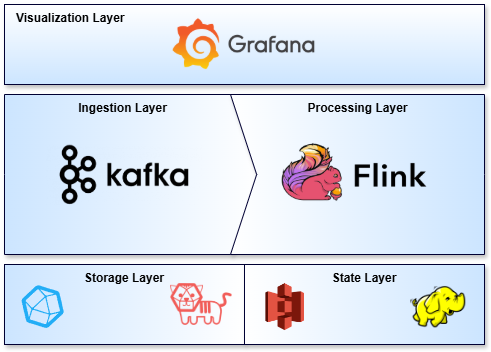
\includegraphics[width=0.99\columnwidth]{graphs/BigDataStack.png}
    \vspace{-0.5cm}
    \caption{Rappresentazione dello stack tecnologico coinvolto.}
    \label{fig:architecture_diagram}
\end{figure}

\subsection{Stack Tecnologico}\label{subsec:big_data_stack}

La pipeline si articola in cinque livelli architetturali principali:

\begin{enumerate}
    \item \textbf{Ingestion Layer}: Il bus dei messaggi distribuito che funge da buffer; disaccoppia la sorgente di dati dal motore di elaborazione e quest'ultimo dal consumatore Telegraf, attutendo i picchi di carico e gestendo in modo trasparente la \emph{backpressure}.
    \item \textbf{Processing Layer}: Il nucleo computazionale del sistema; esegue una topologia distribuita consumando i dati da Kafka ed eseguendo elaborazioni stateful in event-time.
    \item \textbf{State Storage Layer}: Lo storage distribuito deputato al salvataggio dei checkpoint; RocksDB funge da backend di stato locale (in-memory/su disco locale del worker), mentre HDFS garantisce la persistenza distribuita dei backup di stato per la tolleranza ai guasti.
    \item \textbf{Storage Layer}: InfluxDB memorizza sia i risultati analitici che le metriche di runtime di Flink.
    \item \textbf{Visualization Layer}: Fornisce l'interfaccia utente finale per l'osservabilità delle performance del cluster e il monitoraggio degli indicatori analitici del traffico aereo.
\end{enumerate}

% La Tabella~\ref{tab:big_data_stack} riassume i componenti tecnologici impiegati e i rispettivi ruoli nel sistema.
% 
% \begin{table*}[t]
% \centering
% \caption{Lo Stack Tecnologico di Sky Analytics Stream}
% \label{tab:big_data_stack}
% \begin{tabularx}{\textwidth}{l l l X}
% \toprule
% \textbf{Layer} & \textbf{Componente} & \textbf{Tecnologia} & \textbf{Ruolo e Scopo Principale} \\
% \midrule
% \textbf{Ingestion} & Simulatore di Flusso & Go Application & Lettura zero-copy, ordinamento, serializzazione binaria e riproduzione accelerata con disordine % controllato. \\
% \textbf{Message Broker} & Event Bus & Apache Kafka & Disaccoppiamento produttore-consumatore, partizionamento del flusso e storage temporaneo dei risultati. % \\
% \textbf{Processing} & Stream Engine & Apache Flink & Consumo parallelo multi-partizione, calcolo di aggregati in event-time e scrittura su Kafka. \\
% \textbf{State Storage} & Distributed File System & Apache HDFS & Storage durevole e centralizzato per il salvataggio dei checkpoint e savepoint di Flink. \\
% \textbf{Data Integration} & Metrics \& Results Collector & Telegraf Agent & Ingestione automatica dei risultati analitici da Kafka verso InfluxDB. \\
% \textbf{Persistence} & Time-Series DB & InfluxDB v2 & Storicizzazione efficiente dei risultati delle query e telemetria del cluster Flink. \\
% \textbf{Visualization} & Dashboarding UI & Grafana & Visualizzazione real-time delle metriche di traffico aereo e monitoraggio dello stato di salute % dell'infrastruttura. \\
% \bottomrule
% \end{tabularx}
% \end{table*}

\subsection{Flusso dei Dati}\label{subsec:data_flow}

Il ciclo di vita di un singolo evento di volo attraversa sequenzialmente l'intera pipeline (mostrata in Fig.~\ref{fig:interaction_diagram}) seguendo il flusso descritto di seguito:

\begin{enumerate}
    \item \textbf{Generazione e Replay}: Il simulatore legge i dati grezzi dal dataset compresso, gli eventi vengono ordinati, convertiti in JSON e inviati a topic. Qualora configurato, viene applicato l'algoritmo di sfasamento temporale.
    % \item \textbf{Brokeraggio}: Kafka distribuisce i messaggi in ingresso sulle partizioni del topic \texttt{flights-stream}. La scelta di un partizionamento multiplo consente a Flink di leggere i dati in parallelo.
    \item \textbf{Elaborazione}: I TaskManager di Apache Flink consumano lo stream di eventi. Il motore gestisce i watermark in base all'event-time inserito nei record e calcola i risultati per le tre query analitiche concorrenti. Flink emette i risultati intermedi e finali, scrivendoli in specifici topic Kafka di output.
    \item \textbf{Fault-Tolerance}: Durante l'elaborazione, Flink esegue periodicamente checkpoint asincroni. Lo stato locale delle finestre e degli sketch viene sincronizzato su HDFS/S3. % In caso di fallimento di un TaskManager, il JobManager ripristina lo stato dall'ultimo checkpoint valido su HDFS, riavviando il consumo da Kafka dall'offset corretto.
    \item \textbf{Raccolta e Persistenza}: Telegraf ascolta i topic di output di Kafka e converte i messaggi JSON in record pronti per InfluxDB, inserendoli nel bucket dei risultati. Parallelamente, il reporter InfluxDB integrato in Flink invia ogni secondo le metriche di telemetria ad un bucket separato in InfluxDB.
    \item \textbf{Visualizzazione}: Grafana interroga costantemente InfluxDB, aggiornando in tempo reale le visualizzazioni grafiche delle dashboard destinate sia alle metriche applicative sia a quelle infrastrutturali.
\end{enumerate}

\begin{figure}[t]
    \centering
    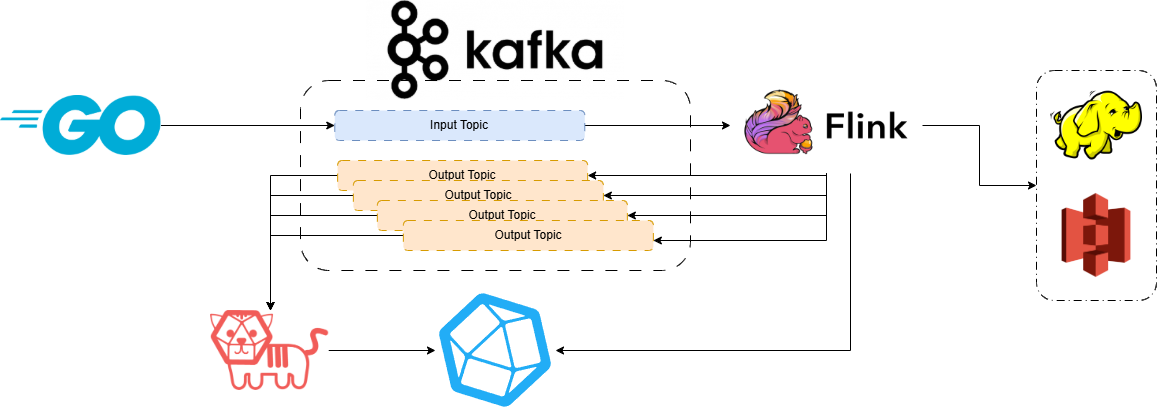
\includegraphics[width=0.99\columnwidth]{graphs/InteractionDiagram}
    \caption{Diagramma di interazione tra le componenti principali della pipeline di Sky Analytics Stream.}
    \label{fig:interaction_diagram}
\end{figure}

% \subsection{Scelte Architetturali Chiave}\label{subsec:architectural_rationale}

% La scelta di questa specifica configurazione architetturale risponde a precisi requisiti ingegneristici:

% \begin{itemize}
%     \item \textbf{Disaccoppiamento tramite Code di Messaggi}: L'uso di Kafka come intermediario protegge Flink da variazioni repentine del throughput di rete o della sorgente. Kafka funge da buffer persistente, consentendo a Flink di consumare i dati alla propria velocità massima stabile ed esercitando contropressione nativa se necessario.
%     \item \textbf{Condivisione della Sorgente}: Anziché lanciare tre job Flink distinti (ognuno dei quali dovrebbe consumare lo stream da Kafka separatamente, decodificare i messaggi JSON ed emettere watermark), le tre query analitiche sono modellate all'interno di un unico DAG. In questo modo si dimezza il carico di I/O su Kafka e si condivide la fase iniziale di parsing ed estrazione del timestamp logico, ottimizzando l'uso di memoria e CPU sui worker.
%     \item \textbf{Archiviazione Stato Ibrida}: La scelta di RocksDB come State Backend consente di gestire uno stato applicativo di dimensioni superiori alla memoria RAM disponibile dei TaskManager, riversando i dati su disco locale. L'integrazione con HDFS garantisce che tali dati siano protetti contro la perdita del singolo host tramite la replica distribuita dei file di checkpoint.
%     \item \textbf{Canale di Output Asincrono per l'Osservabilità}: Flink scrive i risultati su Kafka anziché effettuare chiamate dirette a un database. Questo evita di bloccare i thread di calcolo di Flink con la latenza di scrittura sincrona di un DB, delegando l'inserimento batch a Telegraf e preservando le performance computazionali.
% \end{itemize}

% ------------------------------

\section{Implementazione delle Componenti}\label{sec:implementation_details}

\subsection{Simulatore di Ingestione}\label{subsec:ingestion_simulator}
L'ingestione e il replay degli eventi storici in tempo reale sono gestiti da un componente custom sviluppato in linguaggio Go. La scelta tecnologica è motivata dalla necessità di disporre di un agente di ingestione ad altissime prestazioni, caratterizzato da un consumo minimo di risorse e in grado di garantire throughput elevati senza introdurre colli di bottiglia o latenze spurie dovute alla Garbage Collection (frequenti in ecosistemi basati su JVM).

Per simulare scenari di esecuzione realistici e testare i limiti prestazionali del sistema, sono stati definiti tre scenari di carico basati su diversi fattori di accelerazione temporale, descritti nella Tabella~\ref{tab:go_acceleration_scenarios}. 

Si evidenzia che l'uso dell'accelerazione temporale comporta un aumento del throughput: comprimere il tempo logico riduce drasticamente la durata reale delle finestre temporali di Flink, imponendo una frequenza di trigger e di calcolo dello stato estremamente elevata e artificiale. In uno scenario industriale, qualora si volesse studiare il comportamento del sistema sotto carichi massivi senza tale distorsione, la soluzione ottimale consisterebbe nel sintetizzare dati aggiuntivi (generando nuovi record, anche fittizi, all'interno dello stesso intervallo temporale) in modo da incrementare il throughput mantenendo la durata reale delle finestre vicina a quella reale.

\begin{table}[htbp]
\centering
\caption{Scenari di carico}
\label{tab:go_acceleration_scenarios}
\scriptsize
\setlength{\tabcolsep}{2pt}
\begin{tabular}{lccc}
\toprule
\textbf{Parametro / Metrica} & \textbf{Sce. Basso} & \textbf{Sce. Medio} & \textbf{Sce. Alto} \\
\midrule
\textbf{Moltiplicatore target} & 1.440x & 14.400x & 43.200x \\
\textbf{Fattore tempo log/real} & 1g / 1min & 10g / 1min & 30g / 1min \\
\textbf{Durata del Replay nominale} & $\approx$ 120 min & $\approx$ 12 min & $\approx$ 4 min \\
\textbf{Throughput nominale} & $\approx$ 305 ev/s & $\approx$ 3.050 ev/s & $\approx$ 9.150 ev/s \\
\textbf{Finestra 1h reale} & 2,5 s & 250 ms & 83 ms \\
\midrule
\textbf{Efficienza reale misurata} & $\approx$ 99\% & $\approx$ 96\% & $\approx$ 89\% -- 91\% \\
\textbf{Throughput reale misurato} & $\approx$ 302 ev/s & $\approx$ 2.928 ev/s & $\approx$ 8.140 -- 8.320 ev/s \\
\bottomrule
\end{tabular}
\end{table}

In base a tali scenari di accelerazione, è possibile stimare teoricamente il throughput massimo in uscita atteso per ciascuna delle tre query analitiche, assumendo che non si verifichino scarti o ritardi tardivi tali da innescare emissioni supplementari, come mostrato in Tabella~\ref{tab:max_throughput_expected}. La stima si basa sul numero massimo di chiavi attive e sulla frequenza di chiusura o trigger delle finestre in tempo reale.
% \begin{itemize}
%     \item \textbf{Query 1}: Emette $4$ record (uno per ciascuna compagnia target) alla chiusura di ogni finestra logica di $1$ ora.
%     \item \textbf{Query 2}: Consiste di tre finestre concorrenti. La finestra da $1$ ora e la finestra globale (avente trigger periodico a $1$ ora logica) emettono al massimo % $10$ record ciascuna; la finestra da $6$ ore emette $10$ record ogni $6$ ore logiche (media di $1.67$ record/ora). Il totale teorico è dunque di $21.67$ record per ora % logica.
%     \item \textbf{Query 3}: Composta da tre finestre. Le finestre da $1$ giorno e globale (con trigger a $1$ giorno logico) emettono al massimo $96$ record ciascuna ($4$ % compagnie $\times$ $24$ ore); la finestra da $7$ giorni emette $96$ record ogni $7$ giorni logici (media di $13.71$ record/giorno). Il totale è di $205.71$ record per % giorno logico.
% \end{itemize}

\begin{table}[htbp]
\centering
\caption{Throughput massimo teorico e reale in uscita atteso per ciascuna query}
\label{tab:max_throughput_expected}
\scriptsize
\setlength{\tabcolsep}{2.5pt}
\begin{tabular}{lccc}
\toprule
\textbf{Query / Pipeline} & \textbf{Sce. A (1.440x)} & \textbf{Sce. B (14.400x)} & \textbf{Sce. C (43.200x)} \\
\midrule
\textbf{Query 1} & 1,60 recs/s & 16,00 recs/s & 48,00 recs/s \\
\textbf{Query 2 (1h + 6h + Global)} & 8,67 recs/s & 86,67 recs/s & 260,00 recs/s \\
\textbf{Query 3 (1d + 7d + Global)} & 3,43 recs/s & 34,29 recs/s & 102,86 recs/s \\
\midrule
\textbf{Totale Max Nominale (OUT)} & \textbf{13,70 recs/s} & \textbf{136,96 recs/s} & \textbf{410,86 recs/s} \\
\textbf{Totale Reale Atteso (OUT)} & \textbf{13,56 recs/s} & \textbf{131,48 recs/s} & \textbf{365,66 -- 373,88 recs/s} \\
\bottomrule
\end{tabular}
\end{table}

Si osserva che nella realtà sperimentale, il throughput di Query 2 può risultare inferiore a causa della condizione sul minimo numero di voli in ritardo, che esclude molti aeroporti a bassa frequenza dall'ordinamento Top-10. Al contrario, il throughput reale di Query 3 (o Query 1) può talvolta registrare fluttuazioni positive rispetto a quello teorico a causa della distribuzione degli eventi non uniforme sull'event-time.

Il simulatore implementa diverse funzionalità avanzate e ottimizzazioni ingegneristiche:

\begin{itemize}
    \item \textbf{Ingestione Zero-Copy}: Al primo avvio, il simulatore tenta di localizzare l'archivio compresso del dataset in una directory locale. Qualora non presente, l'applicazione lo scarica automaticamente tramite richiesta HTTP dal server del dipartimento\footnote{\url{http://www.ce.uniroma2.it/courses/sabd2526/project/project-1-data.tar.gz}}. Successivamente, viene verificata l'integrità del file confrontandone l'hash SHA-1 con quello atteso. Una volta superato il controllo, l'archivio originale viene scompattato al volo in memoria, senza la necessità di estrarre preventivamente su disco l'intero dataset in formato CSV. Questo flusso zero-copy riduce al minimo l'uso dello spazio di archiviazione ed elimina i tempi morti dovuti alle operazioni di I/O su disco.
    
    \item \textbf{Binary Caching}: Al fine di minimizzare i tempi di inizializzazione nelle successive esecuzioni, gli eventi letti dal file CSV vengono convertiti in una slice di strutture tipizzate. I record vengono quindi ordinati cronologicamente rispetto al loro event-time logico e serializzati in un file di cache binario locale \texttt{.gob}.
    
    \item \textbf{Gestione del Tempo Fisico}: Il simulatore emula la distanza temporale reale sull'event-time tra i voli applicando il fattore di compressione del tempo ed attendendo la differenza relativa riscalata rispetto all'evento precedente. Con alti fattori di accelerazione (dove le finestre temporali logiche di un'ora si contraggono in pochi millisecondi reali), le funzioni di \textit{sleep} del sistema operativo risulterebbero inadeguate a causa dell'overhead dello scheduler, del kernel e dei \textit{context switch}. Per ovviare a ciò, è stata implementata una strategia di attesa ibrida \textit{Sleep\allowbreak{}-\allowbreak{}Spinlock}: se l'attesa supera la soglia critica \textit{spin threshold} nel file di configurazione, il thread esegue una sleep rilasciando la CPU, mentre al di sotto di tale valore effettua un \textbf{spinlock}. Questo impedisce la sospensione del processo da parte del kernel nel momento critico, garantendo maggiore precisione.
    
    \item \textbf{Out-of-Order Injection}: Al fine di stressare e validare le strategie di Watermarking, la gestione dei dati tardivi di Apache Flink e analizzare il sistema in scenari realistici dove le sorgenti sono diversificate e poco affidabili, il simulatore implementa un decoratore basato su un algoritmo probabilistico. Con una probabilità definita $P \in [0, 1]$, un record viene selezionato e il suo istante di pubblicazione viene dislocato in avanti nel tempo di un offset casuale limitato da un valore massimo configurabile in minuti logici. La sequenza di eventi risultante viene infine ri-ordinata sul tempo di pubblicazione reale prima dell'invio, riproducendo accuratamente i tipici disallineamenti di rete di uno stream distribuito.
    
    % \item \textbf{Pubblicazione su Kafka}: I record sono serializzati in JSON mantenendo i nomi delle colonne e inviati al topic \texttt{flights\allowbreak{}-\allowbreak{}stream} mediante \texttt{kafka\allowbreak{}-\allowbreak{}go}. Il writer usa bilanciamento round-robin, batch fino a 100 messaggi o 100 kB, timeout di 2 ms e modalità asincrona, evitando che la conferma di ogni singolo messaggio alteri la temporizzazione del replay. In alternativa, un sink testuale consente test locali senza Kafka per sviluppo e debugging.
    \item \textbf{Pubblicazione su Kafka}: Il writer usa bilanciamento round-robin, batch fino a 100 messaggi o 100 kB, timeout di 2 ms e modalità asincrona, evitando che la conferma di ogni singolo messaggio alteri la temporizzazione del replay.
\end{itemize}

\subsection{Message Broker}\label{subsec:kafka_integration}

Per disaccoppiare la sorgente dei dati dal motore di stream processing, è stato integrato Apache Kafka come message broker distribuito ad alto throughput. Kafka funge da polmone architetturale, assorbendo le fluttuazioni di carico del flusso in ingresso ed esponendo i dati in modo ordinato e persistente.

\subsubsection{Organizzazione dei Topic e Partizionamento}\label{subsubsec:kafka_topics}
Il flusso di dati in ingresso è gestito tramite il topic principale \texttt{flights-stream}, configurato con $6$ partizioni parallele. Il partizionamento consente di parallelizzare l'elaborazione su più slot di esecuzione di Flink, garantendo la scalabilità orizzontale del sistema.
Per la storicizzazione dei risultati analitici prodotti dalle tre query concorrenti, sono stati definiti diversi topic di output dedicati per ciascuna finestra e granularità temporale. Questo disaccoppia ulteriormente Flink dai database di storage a valle, permettendo a componenti ausiliari come Telegraf di consumare i risultati in modalità asincrona.

\subsubsection{Fase di Ingestione in Flink}\label{subsubsec:kafka_source}
L'integrazione di Kafka come sorgente dati in Flink avviene tramite la classe nativa \texttt{KafkaSource}. 

Per mappare i byte grezzi transitati su Kafka in oggetti Java tipizzati, è stato implementato uno schema di deserializzazione custom. Tale classe esegue le seguenti operazioni per ogni record consumato:
\begin{itemize}
    \item \textbf{Deserializzazione JSON}: converte il messaggio Kafka in un oggetto \texttt{FlightRecord}, scartando i record non validi;
    \item \textbf{Gestione dei timestamp}: assegna al record sia l'event-time del volo sia il tempo di ingestione nel sistema.
\end{itemize}

\subsubsection{Fase di Scrittura dei Risultati}\label{subsubsec:kafka_sink}
Le tre query analitiche concorrenti producono flussi di risultati che vengono re-iniettati in Kafka tramite istanze di \texttt{KafkaSink}, configurate con la garanzia di consegna \textit{at least once} per garantire la tolleranza ai guasti senza l'overhead delle transazioni a due fasi.

La serializzazione da oggetti Java a payload JSON pronti per essere trasmessi in rete è delegata a schemi di serializzazione personalizzati. Ognuno di essi serializza lo stato dell'oggetto in array di byte JSON.

\subsection{Motore di Stream Processing}\label{subsec:flink_component}

Il core computazionale di \textit{Sky Analytics Stream} è realizzato in Apache Flink ed è strutturato in un singolo job distribuito. La topologia a grafo diretto aciclico è orchestrata all'interno della classe principale \texttt{FlightAnalysisJob} e prevede la condivisione a monte della sorgente dei dati e dei filtri di data quality. Questo design a sorgente condivisa riduce al minimo l'I/O ed evita la deserializzazione ridondante dello stream di ingresso.

\subsubsection{Gestione del Disordine Temporale}\label{subsubsec:flink_watermarking}
La riproduzione dei dati può introdurre disallineamenti logici che richiedono strategie di sincronizzazione robuste per l'avanzamento del tempo logico:
\begin{itemize}
    \item \textbf{Watermark}: Viene adottata una strategia configurata con la politica di disordine massimo limitato, parametrizzata tramite il file \texttt{application.yaml}.
    \item \textbf{Idleness Detection}: Per evitare che il blocco o il rallentamento di una delle 6 partizioni di Kafka arresti l'avanzamento del watermark globale dell'intera pipeline, la strategia è irrobustita dall'uso della \textit{idleness}, che esclude temporaneamente dal calcolo le partizioni inattive.
    \item \textbf{Dati Tardivi}: A livello di finestra, viene applicato il metodo \texttt{allowedLateness(d)} per consentire l'aggiornamento tardivo delle metriche qualora giungessero eventi con un ritardo superiore al watermark ma inferiore alla tolleranza aggiuntiva. Per gli eventi che superano anche questa seconda barriera, Flink utilizza un canale di Side Output dedicati per reindirizzare tali record a un analizzatore personalizzato, impedendo che vengano scartati silenziosamente.
\end{itemize}

\subsubsection{Fault Tolerance}\label{subsubsec:flink_checkpointing}
La tolleranza ai guasti e la resilienza del cluster sono gestite tramite il meccanismo di checkpointing distribuito asincrono di Flink (basato sull'algoritmo di Chandy-Lamport):
\begin{itemize}
    \item \textbf{Consistenza Exactly-Once}: Il motore è impostato per garantire che lo stato interno degli operatori venga ripristinato esattamente nello stesso stato pre-fallimento, tramite politica \emph{exactly-once}.
    \item \textbf{State Backend incrementale}: Per evitare colli di bottiglia, lo stato in-flight delle finestre è ospitato su disco locale tramite il backend \textit{RocksDB}. Quest'ultimo scrive le tabelle di stato in file SST locali ed effettua checkpoint incrementali asincroni, garantendo tempi di salvataggio rapidi anche per stati di grandi dimensioni.
    % \item \textbf{Ottimizzazioni anti-saturazione}: La proprietà \texttt{MIN\_PAUSE\_BETWEEN\_CHECKPOINTS} assicura un intervallo di riposo minimo tra la fine di un checkpoint e l'inizio del successivo, eliminando il rischio di saturazione della CPU.
\end{itemize}

\subsubsection{Garanzie di Consegna E2E}\label{subsubsec:flink_delivery_guarantees}
Una delle decisioni architetturali più rilevanti del progetto riguarda il disallineamento pianificato delle garanzie di consegna:
\begin{itemize}
    \item \textbf{At-Least-Once su Kafka}: Il \texttt{SinkBuilder} configura i producer Kafka impostando \textit{at-least-once}. L'implementazione di un sink \textit{exactlyonce} richiederebbe l'attivazione del protocollo a transazioni distribuite di Kafka, il quale introduce un forte overhead di coordinamento.
    \item \textbf{Exactly-Once tramite Idempotenza}: Questa perdita teorica di consistenza sui sink viene completamente compensata a valle da InfluxDB. Poiché InfluxDB è un database temporale che memorizza i punti indicizzati per timestamp e tag-set primari, eventuali messaggi duplicati scritti da Kafka a causa di un ripristino di Flink verranno sovrascritti in modo identico. Questo schema ibrido permette di ottenere la consistenza matematica dell'Exactly-Once end-to-end senza pagare il costo prestazionale delle transazioni distribuite.
\end{itemize}

\subsubsection{DDSketch per i Percentili}\label{subsubsec:flink_ddsketch}
L'algoritmo probabilistico \textbf{DDSketch} è una componente strategica dell'intera architettura, impiegato per risolvere problemi di stima quantilica a memoria costante $O(1)$:
\begin{itemize}
    \item \textbf{Caratteristiche dell'Algoritmo}: DDSketch mappa i valori su indici di bin logaritmici basati su una precisione relativa garantita $\alpha = 0.01$ (garantendo errore massimo dell'1\%). Come evidenziato nel paper originale di Datadog~\cite{masson2019ddsketch}:
    \begin{quote}
        \textit{``...in practice $m$ [the number of bins] is usually set to be a constant large enough to handle a wide range of values. As an example, for $\alpha = 0.01$, a sketch of size 2048 can handle values from 80 microseconds to 1 year, and cover all quantiles.''}
    \end{quote}
    % TODO: inserire solo la citazione senza riporta il testo e descrivere l'algoritmo.
    In conformità con questa analisi teorica, tutte le implementazioni degli accumulatori DDSketch nel nostro progetto (sia analitici che di telemetria) sono state configurate impostando la dimensione massima dello store di bin a $m = 2048$ e l'accuratezza relativa a $\alpha = 0.01$.
    \item \textbf{Dualità d'uso nel Sistema}: DDSketch è stato impiegato con successo in due contesti chiave:
    \begin{enumerate}
        \item \textbf{Distribuzione dei Ritardi}: All'interno dell'accumulatore relativo alla Query 3, DDSketch stima in tempo reale e senza salvare i singoli record in memoria la distribuzione dei ritardi delle compagnie per ciascuna fascia oraria su scale giornaliere, settimanali e globali.
        \item \textbf{Metriche di Latenza Custom}: Per misurare in tempo reale l'efficienza degli operatori e la latenza end-to-end della pipeline, è stato implementato un tracciatore di performance che invia le misurazioni di latenza ad accumulatori basati su DDSketch.
    \end{enumerate}
\end{itemize}

\subsubsection{Sistema di Telemetria}\label{subsubsec:flink_telemetry}
L'osservabilità e il monitoraggio delle performance del sistema in tempo reale si basano su un set di metriche personalizzate registrate tramite la Flink Metric API. Tali metriche si dividono in tre categorie principali:
\begin{itemize}
    \item \textbf{Metriche di Data Quality}: Contatore incrementale ad ogni violazione delle regole di integrità nel filtro di preprocessing.
    \item \textbf{Metriche di Record Tardivi}: All'interno dell'operatore di side-output, vengono registrati il contatore per la quantità di voli arrivati oltre la tolleranza temporale, il gauge di picco storico del ritardo logico e i percentili stimati di latenza dell'event-time.
    \item \textbf{Metriche di Latenza E2E}: Misurate in ogni operatore chiave. Esse includono sia la latenza interna dell'operatore, sia la latenza end-to-end dei dati, stimata su tre orizzonti diversi: rispetto al record più vecchio nella finestra, rispetto al record più recente e rispetto all'istante medio di Ingestion della finestra.
\end{itemize}

A differenza dei risultati di business delle query, le metriche di telemetria hanno un ciclo di vita transitorio ed elevata frequenza di aggiornamento. Di conseguenza, non necessitano di un canale persistente basato su Kafka, il quale comporterebbe solo un inutile overhead di rete ed un inquinamento dei topic con dati estranei all'analitica.

Per ovviare a ciò, il JobManager e i TaskManager di Flink sono configurati nei file di deploy per caricare la classe nativa \texttt{InfluxdbReporterFactory}. Flink stabilisce connessioni dirette verso InfluxDB, inviando periodicamente in modo asincrono le telemetrie di sistema e le metriche custom. % Questa soluzione bypassa interamente Kafka per i dati di monitoraggio, preservando la larghezza di banda del broker per il flusso di ingestion primario e riducendo al minimo la latenza di aggiornamento sulle dashboard di Grafana.

% \subsubsection{Ottimizzazione della Serializzazione}\label{subsubsec:flink_pojo_serialization}
% Per ottimizzare lo scambio di dati sulla rete e le performance di scrittura sul backend di stato, è stata condotta una ristrutturazione architetturale del modello dati % principale:
% \begin{itemize}
%     \item \textbf{Disaccoppiamento del Modello}: La classe \texttt{FlightRecord} è stata spogliata da qualsiasi dipendenza dalle librerie esterne di Kafka e Apache Flink, % isolando lo schema di deserializzazione in un file autonomo (\texttt{FlightRecordDeserializationSchema}). Questo ha reso \texttt{FlightRecord} un \textbf{POJO (Plain Old % Java Object)} puro secondo le convenzioni di Java.
%     \item \textbf{Vantaggi prestazionali di Flink}: Flink utilizza un analizzatore di tipi a runtime. Se una classe rispetta le regole formali dei POJO (costruttore vuoto % pubblico, attributi non-final e metodi getter/setter per ciascun campo), Flink evita di utilizzare la serializzazione generica Kryo, la quale memorizza l'intero grafo di % classe producendo payload voluminosi e costosi in termini di CPU.
%     \item \textbf{Generazione di PojoSerializer}: Flink genera per i POJO dei serializzatori nativi speciali (\texttt{PojoSerializer}), che serializzano solo i byte grezzi dei % dati in modo posizionale fisso. Questo produce due grandi benefici:
%     \begin{enumerate}
%         \item \textbf{Riduzione delle dimensioni dello stato}: Lo stato archiviato in RocksDB è notevolmente più compatto, riducendo i tempi di I/O per i checkpoint asincroni.
%         \item \textbf{Ottimizzazione dei Shuffle di Rete}: Durante le fasi di \texttt{keyBy}, lo shuffle dei record tra i TaskManager su EC2 avviene al massimo throughput % consentito dalla rete, riducendo l'utilizzo di CPU per la codifica/decodifica.
%     \end{enumerate}
% \end{itemize}

\subsubsection{Dettagli delle Query Analitiche ed Ingegnerizzazione del DAG}\label{subsubsec:flink_queries}
\begin{itemize}
    \item \textbf{Query 1}: Filtra i record sui quattro vettori primari tramite \texttt{TargetAirlineFilter} ed effettua una proiezione a basso footprint per ridurre la dimensione dei record prima dello shuffle. Utilizza un aggregatore incrementale per aggiornare lo stato in tempo costante $O(1)$ all'interno di una finestra tumbling di 1 ora in Event-Time.
    \item \textbf{Query 2}: Calcola la top-10 su finestre di 1 ora, 6 ore e globale. Adotta una strategia di classificazione ottimizzata in due fasi logiche: un'aggregazione locale per aeroporto in finestra, seguita da una partizione logica sul timestamp di fine della finestra. Quest'ultima raccoglie le metriche parziali in un \texttt{MapState} locale, registra un timer sul watermark e, al suo scattare, inserisce gli aeroporti idonei in un Min-Heap. Lo stato locale viene ripulito immediatamente dopo l'emissione del risultato per evitare memory leak.
    \item \textbf{Query 3}: Raggruppa gli eventi su chiave composita (basata su \textit{airline} e \textit{hour}) per fasce orarie da 0 a 23 in finestre di 1 giorno, 7 giorni e globale, calcolando i percentili tramite il summenzionato modulo DDSketch.
\end{itemize}

% ------------------------------

\section{Infrastruttura di Deployment}\label{sec:deployment_infrastructure}

La pipeline di \textit{Sky Analytics Stream} è stata progettata per supportare due modalità di esecuzione speculari ma dimensionate diversamente: un deployment locale a container multiplo per sviluppo, e un deployment distribuito multi-nodo su infrastruttura cloud per test prestazionali ed esperimenti di scalabilità.

\subsection{Deployment Locale}\label{subsec:local_deployment}

La configurazione locale consente di validare la correttezza logica del codice e testare il comportamento del sistema in scenari controllati. Viene realizzata tramite un file \texttt{docker-compose.yml} che orchestra undici container connessi a una rete privata bridge:
\begin{itemize}
    \item \textbf{Ingestion \& Broker}: Un container per il broker Kafka e un container di inizializzazione che crea i topic necessari impostandovi il rispettivo partizionamento (6 partizioni per lo stream di ingresso);
    \item \textbf{Stream Processing}: Un container Flink JobManager e tre container TaskManager. Ogni TaskManager dispone di due slot di elaborazione, per un parallelismo massimo locale di 6;
    \item \textbf{State Storage}: Tre container HDFS (un NameNode e due DataNodes) per supportare il salvataggio dei checkpoint in modalità distribuita locale;
    \item \textbf{Persistence \& Telemetry}: Un container InfluxDB (versione \texttt{2.7}) per storicizzare risultati e telemetrie, accoppiato a un container Telegraf che converte i messaggi JSON consumati da Kafka nel modello dati di InfluxDB;
    \item \textbf{Visualization}: Un container Grafana accoppiato a un container \texttt{grafana-image-renderer} (usato per esportare e catturare i grafici delle dashboard).
\end{itemize}

I parametri di configurazione (porte fisiche, credenziali di accesso ai database, token di telemetria e parametri di accelerazione) sono iniettati tramite variabili d'ambiente caricate da un file locale \texttt{.env}.

\subsection{Deployment Distribuito su AWS EC2}\label{subsec:ec2_deployment}

Per condurre le campagne sperimentali in condizioni di carico reale, il sistema è distribuito su un cluster multi-nodo in ambiente cloud Amazon Web Services.

\begin{figure}[h]
    \centering
    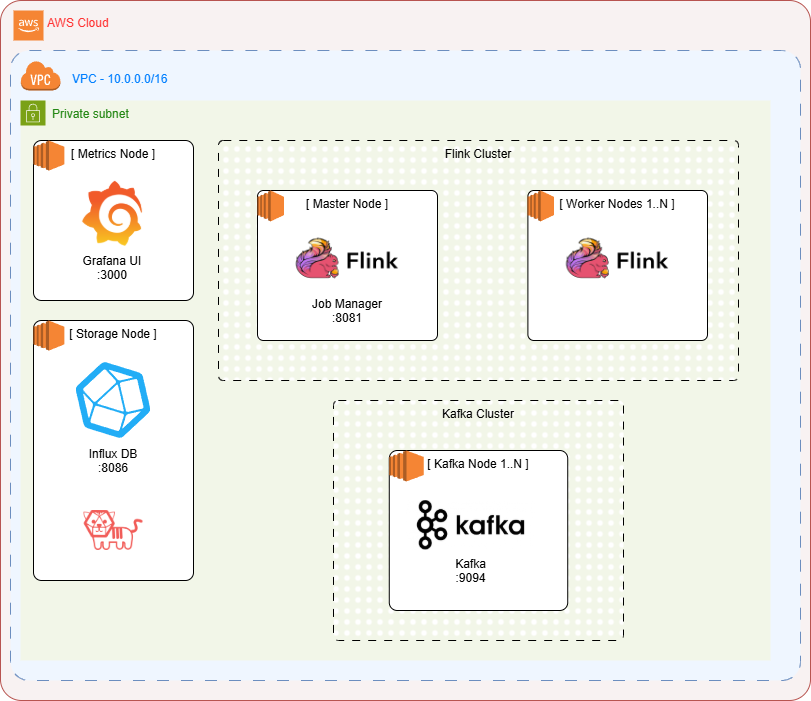
\includegraphics[width=0.90\columnwidth]{graphs/DeploymentView-EC2}
    \caption{Vista architetturale del deployment distribuito su AWS EC2.}
    \label{fig:deployment_ec2}
\end{figure}

\subsubsection{Provisioning dell'Infrastruttura (CloudFormation \& Route 53)}\label{subsubsec:cf_route53}

Il deployment su AWS è automatizzato tramite script che richiamano template di \textbf{AWS CloudFormation}. L'orchestratore esegue le seguenti fasi:
\begin{enumerate}
    \item \textbf{Network Stack}: Crea una VPC dedicata, una sottorete pubblica con CIDR associato, una Security Group con regole di ingresso/uscita per le porte dei servizi, e una \textbf{Private Hosted Zone} su \textbf{Amazon Route 53} con dominio privato \texttt{flight-analysis.local};
    \item \textbf{Bootstrap ed S3}: I pacchetti pre-compilati, i file di configurazione e le variabili d'ambiente vengono caricati su un bucket \textbf{Amazon S3} privato;
    \item \textbf{Node Provisioning}: Lancia le istanze EC2. Ciascun nodo esegue uno script di bootstrap che installa Docker, scarica le configurazioni e i pacchetti dal bucket S3 e avvia i container Docker locali. I nodi vengono registrati automaticamente su Route 53 per consentire la risoluzione dei nomi privati.
\end{enumerate}

\subsubsection{Dimensionamento delle Istanze EC2}\label{subsubsec:ec2_instances}
Il cluster distribuito è composto da istanze EC2 appartenenti alla famiglia general-purpose \texttt{t3} e compute-optimized \texttt{c6i} di AWS\footnote{\url{https://aws.amazon.com/it/ec2/pricing/on-demand/}}, dimensionate per bilanciare i costi con la necessità di risorse CPU e memoria:
\begin{itemize}
    \item \textbf{Kafka Cluster}:
    \begin{itemize}
        \item \emph{Broker 1}: Istanza \textbf{\texttt{t3.large}} (2 vCPU, 8 GiB RAM) per gestire il carico di scrittura primario e avviare il reply del dataset;
        \item \emph{Broker 2 \& 3}: Istanze \textbf{2 x \texttt{t3.medium}} (2 vCPU, 4 GiB RAM) che agiscono come repliche e broker ausiliari.
    \end{itemize}
    \item \textbf{Flink JobManager}: Istanza \textbf{\texttt{c6i.large}} (2 vCPU, 4 GiB RAM) ottimizzata per il calcolo;
    \item \textbf{Flink TaskManagers}: Istanze \textbf{3 x \texttt{c6i.large}} (2 vCPU, 4 GiB RAM) adibite all'esecuzione fisica dei task di Flink (ogni TaskManager ospita 2 slot di calcolo);
    \item \textbf{InfluxDB e Telegraf}: Istanza \textbf{\texttt{t3.small}} (2 vCPU, 2 GiB RAM) per il salvataggio persistente di metriche e risultati;
    \item \textbf{Grafana}: Istanza \textbf{\texttt{t3.small}} (2 vCPU, 2 GiB RAM) per ospitare il servizio di dashboarding;
\end{itemize}

La risoluzione dei nomi DNS privati consente alle macchine di dialogare in modo trasparente senza dover hardcodare gli indirizzi IP pubblici o privati variabili delle istanze.

% ------------------------------

\section{Valutazione Sperimentale}\label{sec:experimental_evaluation}

L'analisi delle prestazioni è suddivisa in tre campagne di test mirate a valutare: l'impatto del parallelismo e la scalabilità, la gestione del disordine temporale e l'impatto del checkpointing con il relativo ripristino in caso di guasti. Tutti i test sono stati condotti sul cluster distribuito AWS EC2 descritto nella Sezione~\ref{subsec:ec2_deployment}.

Si consideri che la velocità di replay effettiva del simulatore Go risente del carico computazionale, dei context switch e dei tempi di I/O del sistema operativo, in particolare sotto elevati fattori di accelerazione temporale si osserva una percentuale di efficienza variabile nel raggiungimento dello speedup target inserito, come mostrato in Tabella~\ref{tab:go_acceleration_scenarios}. Di conseguenza, i throughput in ingresso effettivi misurati su Flink risultano proporzionalmente ridimensionati rispetto ai valori nominali teorici.

\subsection{Parallelismo e Scalabilità in Assenza di Disordine}\label{subsec:perf_parallelism}

La prima campagna di test valuta il comportamento della pipeline al variare del livello di parallelismo, con $P \in \{1, 3, 6\}$, in condizioni di dati ordinati all'origine (disordine aggiuntivo pari a $0$ e tolleranza al ritardo impostata a $0$). Sono confrontati tre livelli di carico riprodotti dal simulatore Go: lo scenario a \textbf{Basso Carico} (moltiplicatore $1.440\times$, throughput nominale $\approx 305$ eventi/secondo), lo scenario a \textbf{Medio Carico} (moltiplicatore $14.400\times$, throughput nominale $\approx 3.050$ eventi/secondo) e lo scenario ad \textbf{Alto Carico} (moltiplicatore $43.200\times$, throughput nominale $\approx 9.150$ eventi/secondo).
\subsubsection{Analisi del Throughput e delle Latenze}\label{subsubsec:throughput_cluster}

L'analisi del throughput e delle latenze a livello di cluster rivela dinamiche prestazionali importanti:
\begin{itemize}
    \item \textbf{Scenario a basso carico}: Il throughput in ingresso oscilla regolarmente intorno a $300$ eventi/s per tutti i livelli di parallelismo, mentre quello complessivo in uscita rimane vicino a $10$ record/s (Figg.~\ref{fig:cluster_throughput_slow_p1}--\ref{fig:cluster_throughput_slow_p6}). La coincidenza delle curve conferma che $P=1$ dispone già di capacità ampiamente sufficiente e che, in questo regime, il parallelismo non produce alcun beneficio di throughput.
    \item \textbf{Throughput in Ingresso e Uscita costante}: A differenza di quanto ci si potrebbe attendere, nello scenario a medio carico il throughput in ingresso reale si attesta costantemente a $\approx 2.900$ eventi/secondo per tutti i livelli di parallelismo. Analogamente, il throughput totale in uscita rimane stabile a $\approx 100$ record/secondo (suddiviso tra Query 1 a $\approx 13$ recs/s, Query 2 a $\approx 58-62$ recs/s e Query 3 a $\approx 27-30$ recs/s). Questo indica che anche un singolo slot è sufficiente a processare l'intero carico dello scenario medio senza accumulare lag su Kafka.
    \item \textbf{Comportamento della latenza Newest P90 al parallelismo 6}: L'analisi del $90$-esimo percentile della latenza \textit{Newest} mostra una stabilità generale intorno ai $5$ secondi per i parallelismi $P=1$ (Fig.~\ref{fig:cluster_latency_medium_p90_p1}) e $P=3$ (Fig.~\ref{fig:cluster_latency_medium_p90_p3}). Al parallelismo $P=6$, tuttavia, a causa della frammentazione del flusso su 6 slot paralleli e del conseguente disallineamento temporaneo dei watermark, si registrano dei picchi transitori: la latenza P90 per la Query 3 7d sale temporaneamente fino a $18,5$ secondi (Fig.~\ref{fig:cluster_latency_medium_p90_p6}), mentre la Query 3 Global mostra un picco di $12,5$ secondi. Questo andamento a impulsi, che poi rientra al baseline di $5$ s, indica disallineamenti temporanei tra i sotto-task di Flink piuttosto che un ritardo cumulativo e permanente.
\end{itemize}

Nel caso a basso carico, sia le latenze medie interne degli operatori sia le curve \textit{Newest P90} rimangono sostanzialmente stabili durante ciascuna esecuzione, senza una crescita progressiva o segnali di accumulo (Figg.~\ref{fig:cluster_latency_slow_p1}--\ref{fig:cluster_latency_slow_p6}). Le finestre lunghe di Query 3 si attestano su livelli diversi rispetto alle query più frequenti; ciò è coerente con la loro minore frequenza di emissione e non costituisce, da solo, un indice di saturazione. Anche i limitati cambi di livello osservabili con $P=6$ sono transitori e non permettono di concludere che il maggiore parallelismo peggiori la latenza. Il risultato supportato dai grafici è quindi più circoscritto: tutti i parallelismi gestiscono stabilmente il basso carico, mentre $P>1$ non offre un beneficio misurabile sul throughput.

Nello scenario ad alto carico, il throughput reale in ingresso si stabilizza per tutte le configurazioni di parallelismo a circa $\approx 8.100 - 8.320$ eventi/secondo. La telemetria della latenza \textit{Newest} (anch'essa valutata sul $90$-esimo percentile per omogeneità di confronto) rivela andamenti stabili:
\begin{itemize}
    \item \textbf{Parallelismi $P=1$ e $P=3$}: Entrambe le configurazioni presentano curve stabili e piatte per l'intera durata dei test. La latenza P90 si attesta costantemente intorno a $2,25$ s (Fig.~\ref{fig:cluster_latency_fast_p90_p1} e Fig.~\ref{fig:cluster_latency_fast_p90_p3}).
    \item \textbf{Parallelismo $P=6$}: La latenza P90 a $P=6$ (Fig.~\ref{fig:cluster_latency_fast_p90_p6}) rimane stabile e controllata intorno a $2$--$2,5$ s per la maggior parte del test, registrando un unico picco transitorio che sale a $6,5$ secondi per la Query 3 7d, prima di stabilizzarsi nuovamente sul livello precedente. Ciò conferma che a P90 gli effetti del watermark drift si traducono in oscillazioni temporanee piuttosto che in accumuli permanenti di ritardo.
\end{itemize}


\subsubsection{Analisi del Consumo delle Risorse}\label{subsubsec:resource_node}

L'incremento del parallelismo mostra un impatto chiaro e positivo sulla distribuzione del carico computazionale (CPU) tra le istanze EC2 attive:
\begin{itemize}
    \item \textbf{Basso carico}: Con $P=1$ il solo worker attivo resta tipicamente intorno allo $0,1$--$0,2\%$ di CPU, con picchi sporadici inferiori all'$1,5\%$ (Fig.~\ref{fig:node_slow_p1}). Con $P=6$, invece, tutti i worker oscillano prevalentemente tra l'$1\%$ e il $5\%$, oltre a un picco di avvio vicino al $25\%$ (Fig.~\ref{fig:node_slow_p6}). A questo livello di traffico il costo di scheduling, serializzazione e coordinamento dei sotto-task domina quindi il lavoro utile; $P=1$ è la configurazione più efficiente.
    \item \textbf{Parallelismo $P=1$}: L'intera elaborazione del DAG di Flink viene allocata su un singolo slot di calcolo di un unico TaskManager. Nello scenario a medio carico, l'istanza \texttt{flink-worker-1} registra un uso di CPU del $\approx 12-16\%$, mentre gli altri worker rimangono inattivi ad uno $0\%$ reale. Nel test ad alto carico (Fig.~\ref{fig:node_cpu_comparison_p1}), l'unico worker attivo \texttt{flink-worker-3} subisce un picco di utilizzo di CPU che oscilla tra il $60\%$ e il $70\%$, rappresentando un punto singolo di potenziale instabilità per l'infrastruttura.
    \item \textbf{Parallelismo $P=3$}: Flink alloca i 3 slot attivi distribuendo il carico su due TaskManager: \texttt{flink-worker-3} registra circa il $45\%$ di CPU nel test ad alto carico, mentre \texttt{flink-worker-2} lavora al $22\%$ CPU. Il terzo worker rimane inutilizzato.
    \item \textbf{Parallelismo $P=6$}: Con tutti i 6 slot del cluster attivi (2 slot per ciascuno dei 3 TaskManager), il carico viene bilanciato in modo eccellente tra tutte e tre le macchine. Nello scenario a medio carico la CPU si attesta uniformemente tra il $10-15\%$, mentre nel test ad alto carico (Fig.~\ref{fig:node_cpu_comparison_p6}) tutte le istanze lavorano in modo cooperativo e simmetrico con un consumo di CPU stabile tra il $20-30\%$.
\end{itemize}

Questo comportamento evidenzia una scalabilità orizzontale dipendente dal carico: negli scenari medio e alto, l'aumento del parallelismo distribuisce i sotto-task e riduce i picchi sul singolo TaskManager; nello scenario lento, invece, la capacità aggiuntiva resta inutilizzata e introduce soltanto overhead di coordinamento. Il parallelismo dovrebbe quindi essere dimensionato rispetto al traffico atteso, anziché mantenuto staticamente al valore massimo.


\subsection{Gestione del Disordine Temporale}\label{subsec:perf_out_of_order}

La seconda campagna di test analizza l'efficacia delle strategie di gestione del disordine temporale (\textit{out-of-orderness}) introdotto dal simulatore Go (con probabilità di ritardo del $5\%$ e ritardo massimo pari a $30$ minuti logici). I test sono stati eseguiti con parallelismo $P=3$, moltiplicatore $14.400\times$, confrontando tre diverse configurazioni di Watermark Delay e Allowed Lateness:
\begin{enumerate}
    \item \textbf{Configurazione Conservativa - $D=30$ min, $L=0$ min}: Privilegia la completezza del dato impostando il ritardo del watermark pari al ritardo massimo teorico dei dati.
    \item \textbf{Configurazione Ibrida - $D=5$ min, $L=25$ min}: Cerca un compromesso emettendo risultati preliminari rapidi e aggiornandoli successivamente per $25$ minuti logici.
    \item \textbf{Configurazione Aggressiva - $D=10$ min, $L=0$ min}: Privilegia la tempestività e la riduzione dell'uso di memoria, scartando i record con ritardo superiore a $10$ minuti.
\end{enumerate}

\subsubsection{Analisi della Perdita di Dati e Accuratezza}\label{subsubsec:data_loss}

L'analisi dei dati evidenzia l'impatto diretto dei parametri sulla completezza del calcolo:
\begin{itemize}
    \item \textbf{Configurazioni Conservativa e Ibrida}: Registrano un numero di record scartati pari a \textbf{zero} (Fig.~\ref{fig:cluster_ooo_d30_l0} e Fig.~\ref{fig:cluster_ooo_d5_l25}). Nella configurazione conservativa, il ritardo di $30$ minuti consente a tutti gli eventi fuori ordine di rientrare prima del passaggio del watermark. Nella configurazione ibrida, sebbene il watermark si muova più rapidamente, la finestra resta attiva in memoria grazie a un' \textit{allowed lateness} di $25$ minuti, garantendo che i voli con ritardo fino a $30$ minuti vengano comunque inclusi nel calcolo finale.
    \item \textbf{Configurazione Aggressiva}: Mostra una significativa perdita di dati. Nel grafico \textit{Record Scartati per Finestra} (Fig.~\ref{fig:cluster_ooo_d10_l0}), si osserva un accumulo continuo di scarti che raggiunge $\approx 970$ record per la Query 2 (finestra 1h), $\approx 590$ record per la Query 1 e $\approx 250$ per la Query 2 (finestra 6h). La distribuzione dei ritardi degli scarti conferma che tutti gli eventi con sfasamento compreso tra $10$ e $30$ minuti sono stati rigettati da Flink, degradando la precisione dei risultati di business.
\end{itemize}

\subsubsection{Trade-off Operativi}\label{subsubsec:latency_tradeoffs}

Le tre strategie comportano trade-off operativi distinti:
\begin{itemize}
    \item \textbf{Latenza di prima emissione}: Nella configurazione conservativa, la latenza di prima emissione è più elevata. La finestra deve attendere $30$ minuti di event-time prima che il watermark superi la fine della finestra stessa e ne causi la chiusura. Nella configurazione ibrida, il primo risultato parziale viene emesso solo dopo $5$ minuti, riducendo drasticamente il tempo di risposta percepito a valle.
    \item \textbf{Carico di Scrittura e Ricalcolo}: La configurazione ibrida, a fronte di una maggiore reattività, genera un carico di I/O considerevole. Ogni record tardivo che giunge dopo la chiusura iniziale della finestra causa la riapertura della stessa, l'esecuzione incrementale degli aggregatori e l'invio di un nuovo record di aggiornamento su Kafka, moltiplicando le scritture. Al contrario, la configurazione conservativa emette un singolo record consolidato per finestra, minimizzando il traffico di rete ed i ricalcoli.
    \item \textbf{Occupazione di Memoria dello Stato}: Nelle configurazioni conservativa e ibrida, Flink deve mantenere in memoria lo stato delle finestre per un tempo prolungato (rispettivamente per $30$ e $25$ minuti logici oltre la fine della finestra). Nella configurazione aggressiva lo stato viene rimosso immediatamente al passaggio del watermark, garantendo un minor consumo di memoria dello State Backend, ma al costo di una perdita di informazioni irreversibile.
\end{itemize}

\subsection{Impatto del Checkpointing}\label{subsec:perf_checkpoint_fault_tolerance}

La terza e ultima campagna di test valuta il comportamento della pipeline Flink in termini di resilienza ed efficienza del meccanismo di tolleranza ai guasti. Le prove sono state condotte con parallelismo $P=6$, moltiplicatore $14.400\times$, senza disordine sorgente aggiunto, confrontando tre differenti scenari:
\begin{enumerate}
    \item \textbf{Scenario 1 - Baseline Checkpoint}: Checkpoint abilitato ogni $5$ minuti, nessun guasto iniettato.
    \item \textbf{Scenario 2 - Valutazione Overhead}: Checkpoint abilitato con frequenza elevata (ogni $30$ secondi), nessun guasto iniettato.
    \item \textbf{Scenario 3 - Test di Ripristino}: Checkpoint ogni $5$ minuti, con iniezione di $1$ fallimento (kill controllato del container del TaskManager \texttt{flink-worker-1}).
\end{enumerate}

La pipeline utilizza RocksDB come State Backend configurato con snapshot incrementali per minimizzare l'I/O di rete verso lo storage distribuito.

\subsubsection{Analisi dell'Overhead del Checkpointing}\label{subsubsec:checkpoint_overhead}

Sebbene in Apache Flink la scrittura del checkpoint sullo storage remoto avvenga in modo asincrono, la frequenza con cui esso viene innescato introduce un costo computazionale legato alla serializzazione dello stato e al coordinamento dei nodi:
\begin{itemize}
    \item \textbf{Dimensione e Durata}: Nello Scenario 1 il completamento di uno snapshot richiede $\approx 2,75$ secondi per uno stato di $\approx 8,20$ MiB. Nello Scenario 2, la durata scende a soli $\approx 474$ ms per uno stato medio di $\approx 4,02$ MiB. Questa drastica riduzione è il risultato diretto degli snapshot incrementali di RocksDB: poiché l'intervallo temporale è ridotto, la quantità di file modificati e copiati su S3 è inferiore.
    \item \textbf{Impatto sul Throughput}: Il throughput reale in ingresso si mantiene stabile alla soglia di regime di $\approx 2.928$ eventi/secondo, mostrando che, in questo caso, l'introduzione di checkpoint più frequenti non intaccano le prestazioni del sistema.
\end{itemize}

% \begin{table}[htbp]
% \centering
% \caption{Analisi dell'Overhead del Checkpointing (Parallelismo $P=6$).}
% \label{tab:checkpoint_overhead}
% \begin{tabular}{p{2.8cm}cc}
% \hline
% \textbf{Metrica} & \textbf{Int. 5 Min} & \textbf{Int. 30 Sec} \\
% \hline
% \textbf{Stato Completato} & 3 Checkpoint & 29 Checkpoint \\
% \textbf{Dimensione Stato} & $\approx 8,20$ MiB & $\approx 4,02$ MiB \\
% \textbf{Durata Checkpoint} & $\approx 2,75$ s & $\approx 474$ ms \\
% \textbf{TM GC Medio} & \textbf{266 ms} & \textbf{431 ms} \\
% \textbf{CPU TM Media} & $\approx 11-13\%$ & $\approx 12-14\%$ \\
% \textbf{Throughput Ingressso} & Stabile a $2.928$ ev/s & Stabile a $2.928$ ev/s \\
% \hline
% \end{tabular}
% \end{table}

\subsubsection{Analisi del Restore}\label{subsubsec:restore_failover}

Nello Scenario 3 viene simulato un guasto critico arrestando brutalmente l'istanza \texttt{flink-worker-1}. Le metriche a livello di cluster (Fig.~\ref{fig:cluster_throughput_int5_fail1} e Fig.~\ref{fig:cluster_latency_int5_fail1}) e di nodo (Fig.~\ref{fig:node_chk_run_int5_fail1}) mostrano la sequenza esatta degli eventi:
\begin{itemize}
    \item \textbf{Rilevamento e Downtime}: Non appena il JobManager rileva l'assenza del TaskManager, interrompe immediatamente il Job. Il throughput in ingresso e uscita crolla a zero per un tempo di failover $T_{\text{failover}} \approx 15$ secondi logici reali. In questo intervallo il JobManager re-alloca la topologia distribuita sugli slot rimanenti e sul worker riavviato.
    \item \textbf{Rollback dello Stato consistente}: Flink ripristina lo stato del Job recuperando i dati di business e i metadati dall'ultimo checkpoint consistente valido reimpostando i contatori e le finestre attive a quel preciso istante logico.
    \item \textbf{Fase di Catch-up}: Durante il fermo di 15 secondi, il simulatore Go ha continuato ad inviare voli su Kafka, accumulando lag. Al riavvio, la sorgente Flink consuma i messaggi accumulati al massimo delle sue capacità. Il throughput in ingresso subisce una brusca impennata toccando un picco di $\approx 9.000$ eventi/secondo, mentre in uscita il throughput di scrittura tocca temporaneamente i $250$ record/secondo.
    \item \textbf{Impennata della CPU}: Per elaborare la mole di dati accumulata, il TaskManager riattivato \texttt{flink-worker-1} registra un picco di utilizzo della CPU che tocca il $60\%$ (Fig.~\ref{fig:node_chk_run_int5_fail1}).
    \item \textbf{Picco e Rientro delle Latenze}: Poiché i record processati durante la ripartenza hanno stazionato a lungo su Kafka, la loro latenza end-to-end aumenta significativamente, con un picco della latenza \textit{Average} che sale fino a $2$ minuti. Una volta azzerato il lag accumulato, l'elaborazione ritorna in tempo reale e le latenze rientrano nei valori tipici.
\end{itemize}

Questo test dimostra la robustezza dell'architettura: il sistema ripristina la corretta elaborazione senza perdita osservata di eventi né duplicazioni visibili nei risultati. Flink garantisce consistenza \textit{exactly-once} fino allo stato interno; sul tratto Kafka--InfluxDB, configurato \textit{at-least-once}, l'idempotenza delle scritture con la medesima chiave e timestamp di finestra rende innocue le duplicazioni prodotte durante il ripristino. La garanzia end-to-end dipende quindi dal mantenimento di tale schema di chiavi.

\subsection{Analisi dei Risultati Analtici}\label{subsec:analytical_results}

Oltre alle metriche infrastrutturali, sono stati osservati i risultati di business prodotti dalle tre query, confrontando il dataset completo con la versione soggetta a una perdita casuale degli eventi. I grafici completi sono riportati nell'Appendice~\ref{subsec:appendix_analytical_results}.

\paragraph{Query 1 -- prestazioni delle compagnie.}
Le serie orarie mostrano una marcata variabilità temporale: i ritardi medi restano generalmente nell'ordine di pochi minuti, ma presentano picchi concentrati in specifici giorni, coerenti con episodi operativi circoscritti. Anche il tasso di cancellazione è intermittente e alterna lunghi periodi prossimi allo zero a picchi locali. Tale co-occorrenza suggerisce che le criticità non siano distribuite uniformemente nel quadrimestre. Il confronto tra le quattro compagnie evidenzia profili differenti, ma la posizione dei picchi principali rimane sostanzialmente invariata nel caso con perdita (Figg.~\ref{fig:q1_aa_complete}--\ref{fig:q1_wn_loss}).

\paragraph{Query 2 -- aeroporti con ritardi severi.}
La graduatoria globale è dominata dagli aeroporti con identificativo 11298, 11292, 10397 e 13930, che nel dataset completo totalizzano rispettivamente 15.979, 13.629, 13.430 e 12.315 ritardi severi. Nelle finestre brevi la classifica è invece più volatile: l'ultima finestra di un'ora contiene poche decine di voli e solo due aeroporti superano la soglia di ammissibilità, mentre la finestra di sei ore restituisce una top-10 più stabile. Il risultato mette in luce un effetto importante della granularità: le finestre brevi sono più reattive, ma anche più sensibili alla casualità campionaria; la finestra globale identifica con maggiore affidabilità gli hub strutturalmente critici (Figg.~\ref{fig:q2_1h_complete}--\ref{fig:q2_global_loss}).

\paragraph{Query 3 -- distribuzione dei ritardi.}
Per tutte le compagnie la distanza tra mediana e percentile 90, insieme a massimi di molte ore, conferma una distribuzione fortemente asimmetrica a destra: la maggioranza dei voli parte in orario o con ritardi contenuti, mentre una piccola coda di eventi estremi determina gran parte della variabilità. Il profilo per ora del giorno rende inoltre visibile un peggioramento nelle fasce pomeridiane e serali, compatibile con la propagazione dei ritardi lungo le rotazioni giornaliere. Per WN, ad esempio, nella finestra globale si osservano $p_{25}\approx-4,35$ min, mediana prossima allo zero, $p_{75}\approx11$ min e $p_{90}\approx33,6$ min, a fronte di un massimo di circa 12 ore (Figg.~\ref{fig:q3_wn_global_complete} e~\ref{fig:q3_wn_global_loss}).

\paragraph{Effetto della perdita.}
Il confronto visuale mostra che trend, picchi principali, ordinamento degli aeroporti e profili dei percentili restano molto simili. La perdita casuale riduce la numerosità disponibile e può modificare marginalmente conteggi e posizioni vicine in classifica, ma non introduce uno scostamento sistematico evidente nelle metriche normalizzate, quali media, tasso di cancellazione e percentili. Questo comportamento è plausibile quando la perdita è approssimativamente uniforme e indipendente dal valore del ritardo. Non equivale però a dimostrare l'assenza di bias: una perdita correlata a compagnia, aeroporto, fascia oraria o severità del ritardo potrebbe alterare sensibilmente i risultati.

% ------------------------------

\section{Conclusioni e Sviluppi Futuri}\label{sec:conclusions_future_work}

Il progetto ha realizzato una pipeline distribuita completa per l'analisi in event-time del traffico aereo, integrando simulazione accelerata, Kafka, Apache Flink, persistenza su InfluxDB e osservabilità tramite Grafana. Le prove mostrano che il sistema sostiene circa $300$ eventi/s nello scenario lento, $2.900$ eventi/s nello scenario medio e oltre $8.000$ eventi/s nello scenario ad alto carico, senza accumulo permanente di ritardo. L'aumento del parallelismo non incrementa il throughput, limitato dalla sorgente: ai carichi medio e alto distribuisce il lavoro e riduce i picchi sul singolo nodo, mentre a basso carico mantiene latenze stabili ma non offre vantaggi prestazionali misurabili.

La campagna sul disordine temporale conferma che watermark e \textit{allowed lateness} devono essere dimensionati congiuntamente: le configurazioni conservativa e ibrida preservano la completezza, mentre quella aggressiva riduce lo stato mantenuto ma scarta gli eventi oltre la soglia. Il checkpointing incrementale introduce un overhead contenuto; in presenza di guasto, il sistema completa il ripristino, assorbe il backlog Kafka e torna al regime ordinario. I risultati analitici mostrano inoltre che ritardi e cancellazioni sono concentrati temporalmente e che le distribuzioni dei ritardi hanno code destre pronunciate. Una perdita casuale non altera visibilmente le conclusioni aggregate, pur riducendo la confidenza sulle finestre meno popolate.

Gli sviluppi futuri più utili riguardano una valutazione statistica ripetuta della perdita dati, test di carico capaci di saturare effettivamente Flink e un confronto tra politiche di watermark adattive.

\begin{thebibliography}{10}

\bibitem{fernando2023quantiles}
L.~Fernando, H.~Bindra, and K.~Daudjee, ``An experimental analysis of quantile sketches over data streams,'' in \emph{Proceedings of the 26th International Conference on Extending Database Technology (EDBT '23)}, pp. 1--12, 2023.

\bibitem{masson2019ddsketch}
C.~Masson, J.~E. Rim, and H.~K. Lee, ``DDSketch: A fast and fully-mergeable quantile sketch with relative-error guarantees,'' \emph{Proceedings of the VLDB Endowment}, vol. 12, no. 12, pp. 2195--2205, 2019.

\end{thebibliography}

\clearpage
\onecolumn

\clearpage

\appendices

\section{Utilizzo di strumenti di Intelligenza Artificiale Generativa}\label{sec:appendix_ai_declaration}

Durante lo svolgimento del progetto, gli strumenti di IA generativa sono stati impiegati principalmente come supporto per velocizzare la scrittura di codice boilerplate, l'ottimizzazione sintattica di parti ripetitive di configurazione e per il raffinamento formale del testo della relazione e dei commenti descrittivi. 
Il principale strumento utilizzato è stato Gemini, impiegato sia in versione chatbot che mediante interfacce di programmazione.

Anche i refactoring orientati a migliorare la manutenibilità e la leggibilità del codice sorgente sono stati eseguiti con il supporto di tali modelli, ma sono sempre stati guidati in modo deterministico attraverso prompt specifici. 
In tali istruzioni veniva descritta in maniera estremamente dettagliata la topologia e l'architettura logica finale desiderata per il software, senza mai delegare allo strumento decisioni critiche o scelte algoritmiche volte a definire i componenti del sistema. Queste ultime sono state ideate in modo del tutto autonomo prima della generazione sintattica.

L'intero design del sistema, la logica computazionale delle query analitiche, l'integrazione tra i framework e le scelte metodologiche implementate non sono in alcun modo frutto di decisioni delegate all'AI, ma derivano esclusivamente da un lavoro di progettazione indipendente. 
Nessun concetto chiave riguardante il partizionamento dei flussi su Apache Kafka, le politiche di watermarking e la gestione dei dati tardivi su Apache Flink, la strutturazione logica degli accumulatori basati sull'algoritmo probabilistico DDSketch, la gestione dello stato incrementale tramite RocksDB o i meccanismi di tolleranza ai guasti e di consistenza end-to-end è stato impostato o risolto dai modelli generativi; l'utilità di questi ultimi si è limitata alla mera traduzione sintattica di direttive architetturali preventivamente stabilite dagli autori.

Nello specifico, abbiamo sfruttato questi strumenti per:

\begin{itemize}
    \item \textbf{Codice ripetitivo e boilerplate:} Generazione automatica di componenti software standardizzate che avrebbero richiesto tempi prolungati di scrittura manuale senza apportare valore logico aggiunto. Ciò include la generazione di metodi getter/setter, costruttori e la configurazione iniziale di classi Java strutturate secondo le convenzioni POJO al fine di garantire l'ottimizzazione nativa del \texttt{PojoSerializer} di Flink; la stesura di tali classi è avvenuta esclusivamente a valle di una definizione a priori dello schema dati e dei parametri necessari al funzionamento logico del software, stabiliti in totale autonomia.
    \item \textbf{File di configurazione e schemi:} Compilazione di sezioni sintattiche ripetitive all'interno dei file di configurazione, con particolare riferimento alla mappatura delle variabili d'ambiente per l'orchestrazione multi-container in \texttt{docker-compose.yml} e per i file di deployment.
    \item \textbf{Refactoring e commenti del codice:} Ottimizzazione della leggibilità e della pulizia del codice sorgente attraverso la ristrutturazione formale di blocchi complessi e l'inserimento sistematico di commenti strutturati in standard Javadoc, operando esclusivamente sulla forma espressiva e mai sulla logica algoritmica.
    \item \textbf{Raffinamento linguistico della relazione:} Revisione stilistica, ortografica e lessicale del testo del report accademico. L'intero documento è stato redatto integralmente a mano e, successivamente, sottoposto a una riformulazione guidata tramite modelli di linguaggio al fine di elevare il registro formale richiesto dallo standard IEEE, garantendo l'assoluta invarianza, fedeltà e paternità dei contenuti analitici ed espressivi originari.
    \item \textbf{Infrastruttura di deployment cloud:} Supporto nella stesura sintattica delle sezioni ripetitive dei template di automazione AWS CloudFormation e dei relativi script di bootstrap delle istanze EC2. Una volta definita, dimensionata e testata manualmente l'architettura ottimale del cluster distribuito, l'ausilio dell'AI è stato finalizzato alla traduzione di tale topologia in codice infrastrutturale, automatizzando la scrittura delle componenti standard necessarie.
\end{itemize}

La fase di debugging generale e di ottimizzazione prestazionale del sistema ha visto un ricorso sporadico e mirato agli strumenti di IA generativa. 
Tale supporto si è rivelato utile esclusivamente nei casi in cui i log di tracciamento o gli output degli errori distribuiti forniti risultavano complessi o poco dettagliati. 
Attraverso l'interrogazione dei modelli è stato possibile analizzare più rapidamente le cause radice di tali anomalie sintattiche o di configurazione sistemistica, procedendo poi all'ideazione e all'implementazione puramente manuale della soluzione logica ed ingegneristica necessaria a risolverle.

Ogni singolo blocco di codice, configurazione o direttiva infrastrutturale derivante da tutte queste attività è stato comunque analizzato riga per riga, verificato nella sintassi, integrato all'interno del sistema e validato sperimentalmente attraverso le campagne di test per assicurarne l'assoluta correttezza, l'efficienza e la totale aderenza ai requisiti del progetto.

\clearpage

\section{Rappresentazioni Grafiche e Allegati}\label{sec:appendix_graphics}

In questa appendice sono raccolti i grafici di telemetria estratti da Grafana relativi alle campagne di test descritte nella Sezione~\ref{sec:experimental_evaluation}.

\subsection{Parallelismo e Scalabilità}

% --------------
%   THROUGHPUT  
% --------------

\throughputChart{cluster_clean_run_slow_para1_part6}{Throughput del cluster per lo scenario a basso carico con parallelismo $P=1$.}{fig:cluster_throughput_slow_p1}

\throughputChart{cluster_clean_run_slow_para3_part6}{Throughput del cluster per lo scenario a basso carico con parallelismo $P=3$.}{fig:cluster_throughput_slow_p3}

\throughputChart{cluster_clean_run_slow_para6_part6}{Throughput del cluster per lo scenario a basso carico con parallelismo $P=6$.}{fig:cluster_throughput_slow_p6}

\throughputChart{cluster_clean_run_medium_para1_part6}{Throughput del cluster per lo scenario a medio carico con parallelismo $P=1$.}{fig:cluster_throughput_medium_p1}

\throughputChart{cluster_clean_run_medium_para3_part6}{Throughput del cluster per lo scenario a medio carico con parallelismo $P=3$.}{fig:cluster_throughput_medium_p3}

\throughputChart{cluster_clean_run_medium_para6_part6}{Throughput del cluster per lo scenario a medio carico con parallelismo $P=6$.}{fig:cluster_throughput_medium_p6}

\throughputChart{cluster_clean_run_fast_para1_part6}{Throughput del cluster per lo scenario a alto carico con parallelismo $P=1$.}{fig:cluster_throughput_fast_p1}

\throughputChart{cluster_clean_run_fast_para3_part6}{Throughput del cluster per lo scenario a alto carico con parallelismo $P=3$.}{fig:cluster_throughput_fast_p3}

\throughputChart{cluster_clean_run_fast_para6_part6}{Throughput del cluster per lo scenario a alto carico con parallelismo $P=6$.}{fig:cluster_throughput_fast_p6}


% -------------
%    LATENZA   
% -------------

\latencyChart{cluster_clean_run_slow_para1_part6}{Latenza end-to-end P90 per lo scenario a basso carico con parallelismo $P=1$.}{fig:cluster_latency_slow_p1}

\latencyChart{cluster_clean_run_slow_para3_part6}{Latenza end-to-end P90 per lo scenario a basso carico con parallelismo $P=3$.}{fig:cluster_latency_slow_p3}

\latencyChart{cluster_clean_run_slow_para6_part6}{Latenza end-to-end P90 per lo scenario a basso carico con parallelismo $P=6$.}{fig:cluster_latency_slow_p6}

\latencyChart{cluster_clean_run_medium_para1_part6}{Latenza end-to-end P90 per lo scenario a medio carico con parallelismo $P=1$.}{fig:cluster_latency_medium_p90_p1}

\latencyChart{cluster_clean_run_medium_para3_part6}{Latenza end-to-end P90 per lo scenario a medio carico con parallelismo $P=3$.}{fig:cluster_latency_medium_p90_p3}

\latencyChart{cluster_clean_run_medium_para6_part6}{Latenza end-to-end P90 per lo scenario a medio carico con parallelismo $P=6$.}{fig:cluster_latency_medium_p90_p6}

\latencyChart{cluster_clean_run_fast_para1_part6}{Latenza end-to-end P90 per lo scenario a alto carico con parallelismo $P=1$.}{fig:cluster_latency_fast_p90_p1}

\latencyChart{cluster_clean_run_fast_para3_part6}{Latenza end-to-end P90 per lo scenario a alto carico con parallelismo $P=3$.}{fig:cluster_latency_fast_p90_p3}

\latencyChart{cluster_clean_run_fast_para6_part6}{Latenza end-to-end P90 per lo scenario a alto carico con parallelismo $P=6$.}{fig:cluster_latency_fast_p90_p6}

% -------------
% RISORSE NODO 
% -------------

\nodeChart{node_clean_run_slow_para1_part6}{Utilizzo delle risorse per nodo a basso carico con parallelismo $P=1$.}{fig:node_slow_p1}

\nodeChart{node_clean_run_slow_para3_part6}{Utilizzo delle risorse per nodo a basso carico con parallelismo $P=3$.}{fig:node_slow_p3}

\nodeChart{node_clean_run_slow_para6_part6}{Utilizzo delle risorse per nodo a basso carico con parallelismo $P=6$.}{fig:node_slow_p6}

\nodeChart{node_clean_run_fast_para1_part6}{Utilizzo risorse per nodo (medio/alto carico) con parallelismo $P=1$.}{fig:node_cpu_comparison_p1}

\nodeChart{node_clean_run_medium_para1_part6}{Utilizzo delle risorse per nodo a medio carico con parallelismo $P=1$.}{fig:node_medium_p1}

\nodeChart{node_clean_run_medium_para3_part6}{Utilizzo delle risorse per nodo a medio carico con parallelismo $P=3$.}{fig:node_medium_p3}

\nodeChart{node_clean_run_medium_para6_part6}{Utilizzo delle risorse per nodo a medio carico con parallelismo $P=6$.}{fig:node_medium_p6}

\nodeChart{node_clean_run_fast_para3_part6}{Utilizzo delle risorse per nodo ad alto carico con parallelismo $P=3$.}{fig:node_fast_p3}

\nodeChart{node_clean_run_fast_para6_part6}{Utilizzo risorse per nodo (medio/alto carico) con parallelismo $P=6$.}{fig:node_cpu_comparison_p6}


\subsection{Gestione del Disordine}

% --------------
%   THROUGHPUT  
% --------------

\throughputChart{cluster_delay_run_d30_l0}{Throughput del cluster per lo scenario con delay $D=30$ e latenza $L=0$.}{fig:cluster_throughput_d30_l0}

\throughputChart{cluster_delay_run_d5_l25}{Throughput del cluster per lo scenario con delay $D=5$ e latenza $L=25$.}{fig:cluster_throughput_d5_l25}

\throughputChart{cluster_delay_run_d10_l0}{Throughput del cluster per lo scenario con delay $D=10$ e latenza $L=0$.}{fig:cluster_throughput_d10_l0}

% -------------
%    LATENZA   
% -------------

\latencyChart{cluster_delay_run_d30_l0}{Latenza end-to-end P90 per lo scenario con delay $D=30$ e latenza $L=0$.}{fig:cluster_latency_d30_l0}

\latencyChart{cluster_delay_run_d5_l25}{Latenza end-to-end P90 per lo scenario con delay $D=5$ e latenza $L=25$.}{fig:cluster_latency_d5_l25}

\latencyChart{cluster_delay_run_d10_l0}{Latenza end-to-end P90 per lo scenario con delay $D=10$ e latenza $L=0$.}{fig:cluster_latency_d10_l0}

% -------------
%   DISORDINE  
% -------------

\outoforderChart{cluster_delay_run_d30_l0}{Out-of-orderness per lo scenario con delay $D=30$ e latenza $L=0$.}{fig:cluster_ooo_d30_l0}

\outoforderChart{cluster_delay_run_d5_l25}{Out-of-orderness per lo scenario con delay $D=5$ e latenza $L=25$.}{fig:cluster_ooo_d5_l25}

\outoforderChart{cluster_delay_run_d10_l0}{Out-of-orderness per lo scenario con delay $D=10$ e latenza $L=0$.}{fig:cluster_ooo_d10_l0}

% -------------
% RISORSE NODO
% -------------

\nodeChart{node_delay_run_d30_l0}{Utilizzo delle risorse per nodo con watermark delay $D=30$ min e allowed lateness $L=0$.}{fig:node_delay_d30_l0}

\nodeChart{node_delay_run_d5_l25}{Utilizzo delle risorse per nodo con watermark delay $D=5$ min e allowed lateness $L=25$ min.}{fig:node_delay_d5_l25}

\nodeChart{node_delay_run_d10_l0}{Utilizzo delle risorse per nodo con watermark delay $D=10$ min e allowed lateness $L=0$.}{fig:node_delay_d10_l0}


\subsection{Checkpointing e Resilienza}

% --------------
%   THROUGHPUT  
% --------------

\throughputChart{cluster_chk_run_int30_fail0}{Throughput del cluster per lo scenario con checkpointing ogni $30$ secondi e con 0 fallimenti.}{fig:cluster_throughput_int30_fail0}

\throughputChart{cluster_chk_run_int5_fail0}{Throughput del cluster per lo scenario con checkpointing ogni $5$ minuti e con 0 fallimenti.}{fig:cluster_throughput_int5_fail0}

\throughputChart{cluster_chk_run_int5_fail1}{Throughput del cluster per lo scenario con checkpointing ogni $5$ minuti e con 1 fallimento.}{fig:cluster_throughput_int5_fail1}

% -------------
%    LATENZA   
% -------------

\latencyChart{cluster_chk_run_int30_fail0}{Latenza end-to-end P90 per lo scenario con checkpointing ogni $30$ secondi e con 0 fallimenti.}{fig:cluster_latency_int30_fail0}

\latencyChart{cluster_chk_run_int5_fail0}{Latenza end-to-end P90 per lo scenario con checkpointing ogni $5$ minuti e con 0 fallimenti.}{fig:cluster_latency_int5_fail0}

\latencyChart{cluster_chk_run_int5_fail1}{Latenza end-to-end P90 per lo scenario con checkpointing ogni $5$ minuti e con 1 fallimento.}{fig:cluster_latency_int5_fail1}

% -------------
%    LATENZA   
% -------------

\checkpointChart{cluster_chk_run_int30_fail0}{Checkpointing del cluster per lo scenario con checkpointing ogni $30$ secondi e con 0 fallimenti.}{fig:cluster_chk_int30_fail0}

\checkpointChart{cluster_chk_run_int5_fail0}{Checkpointing del cluster per lo scenario con checkpointing ogni $5$ minuti e con 0 fallimenti.}{fig:cluster_chk_int5_fail0}

\checkpointChart{cluster_chk_run_int5_fail1}{Checkpointing del cluster per lo scenario con checkpointing ogni $5$ minuti e con 1 fallimento.}{fig:cluster_chk_int5_fail1}

% -------------
%   DISORDINE  
% -------------

\outoforderChart{cluster_chk_run_int30_fail0}{Out-of-orderness per lo scenario con checkpointing ogni $30$ secondi e con 0 fallimenti.}{fig:cluster_ooo_int30_fail0}

\outoforderChart{cluster_chk_run_int5_fail0}{Out-of-orderness per lo scenario con checkpointing ogni $5$ minuti e con 0 fallimenti.}{fig:cluster_ooo_int5_fail0}

\outoforderChart{cluster_chk_run_int5_fail1}{Out-of-orderness per lo scenario con checkpointing ogni $5$ minuti e con 1 fallimento.}{fig:cluster_ooo_int5_fail1}

% -------------
% RISORSE NODO 
% -------------

\nodeChart{node_chk_run_int5_fail1}{Utilizzo delle risorse per nodo per lo scenario con checkpointing ogni 5 minuti e con 1 fallimento.}{fig:node_chk_run_int5_fail1}

\nodeChart{node_chk_run_int30_fail0}{Utilizzo delle risorse per nodo per lo scenario con checkpointing ogni 30 secondi e con 0 fallimento.}{fig:node_chk_int30_fail0}

\nodeChart{node_chk_run_int5_fail0}{Utilizzo delle risorse per nodo per lo scenario con checkpointing ogni 5 minuti e con 0 fallimenti.}{fig:node_chk_int5_fail0}

\clearpage
\subsection{Risultati delle Query Analitiche}\label{subsec:appendix_analytical_results}

I grafici sono organizzati per scenario: viene presentato prima l'insieme completo dei risultati e, successivamente, l'insieme ottenuto con una perdita casuale degli eventi.

\queryOneChart{Q1_AA_l0.png}{Query 1, dataset completo, American Airlines (AA): ritardo medio e tasso di cancellazione.}{fig:q1_aa_complete}
\queryOneChart{Q1_DL_l0.png}{Query 1, dataset completo, Delta Air Lines (DL): ritardo medio e tasso di cancellazione.}{fig:q1_dl_complete}
\queryOneChart{Q1_UA_l0.png}{Query 1, dataset completo, United Airlines (UA): ritardo medio e tasso di cancellazione.}{fig:q1_ua_complete}
\queryOneChart{Q1_WN_l0.png}{Query 1, dataset completo, Southwest Airlines (WN): ritardo medio e tasso di cancellazione.}{fig:q1_wn_complete}

\queryOneChart{Q1_AA_l10.png}{Query 1, dataset con perdita, American Airlines (AA): ritardo medio e tasso di cancellazione.}{fig:q1_aa_loss}
\queryOneChart{Q1_DL_l10.png}{Query 1, dataset con perdita, Delta Air Lines (DL): ritardo medio e tasso di cancellazione.}{fig:q1_dl_loss}
\queryOneChart{Q1_UA_l10.png}{Query 1, dataset con perdita, United Airlines (UA): ritardo medio e tasso di cancellazione.}{fig:q1_ua_loss}
\queryOneChart{Q1_WN_l10.png}{Query 1, dataset con perdita, Southwest Airlines (WN): ritardo medio e tasso di cancellazione.}{fig:q1_wn_loss}

\queryTwoOneHourChart{Q2_l0.png}{Query 2, dataset completo: classifica sulla finestra di un'ora.}{fig:q2_1h_complete}
\queryTwoSixHourChart{Q2_l0.png}{Query 2, dataset completo: classifica sulla finestra di sei ore.}{fig:q2_6h_complete}
\queryTwoGlobalChart{Q2_l0.png}{Query 2, dataset completo: classifica sulla finestra globale.}{fig:q2_global_complete}

\queryTwoOneHourChart{Q2_l10.png}{Query 2, dataset con perdita: classifica sulla finestra di un'ora.}{fig:q2_1h_loss}
\queryTwoSixHourChart{Q2_l10.png}{Query 2, dataset con perdita: classifica sulla finestra di sei ore.}{fig:q2_6h_loss}
\queryTwoGlobalChart{Q2_l10.png}{Query 2, dataset con perdita: classifica sulla finestra globale.}{fig:q2_global_loss}

\queryThreeOneDayChart{Q3_AA_l0.png}{Query 3, dataset completo, AA: finestra di un giorno.}{fig:q3_aa_1d_complete}
\queryThreeSevenDayChart{Q3_AA_l0.png}{Query 3, dataset completo, AA: finestra di sette giorni.}{fig:q3_aa_7d_complete}
\queryThreeGlobalChart{Q3_AA_l0.png}{Query 3, dataset completo, AA: finestra globale.}{fig:q3_aa_global_complete}
\queryThreeOneDayChart{Q3_DL_l0.png}{Query 3, dataset completo, DL: finestra di un giorno.}{fig:q3_dl_1d_complete}
\queryThreeSevenDayChart{Q3_DL_l0.png}{Query 3, dataset completo, DL: finestra di sette giorni.}{fig:q3_dl_7d_complete}
\queryThreeGlobalChart{Q3_DL_l0.png}{Query 3, dataset completo, DL: finestra globale.}{fig:q3_dl_global_complete}
\queryThreeOneDayChart{Q3_UA_l0.png}{Query 3, dataset completo, UA: finestra di un giorno.}{fig:q3_ua_1d_complete}
\queryThreeSevenDayChart{Q3_UA_l0.png}{Query 3, dataset completo, UA: finestra di sette giorni.}{fig:q3_ua_7d_complete}
\queryThreeGlobalChart{Q3_UA_l0.png}{Query 3, dataset completo, UA: finestra globale.}{fig:q3_ua_global_complete}
\queryThreeOneDayChart{Q3_WN_l0.png}{Query 3, dataset completo, WN: finestra di un giorno.}{fig:q3_wn_1d_complete}
\queryThreeSevenDayChart{Q3_WN_l0.png}{Query 3, dataset completo, WN: finestra di sette giorni.}{fig:q3_wn_7d_complete}
\queryThreeGlobalChart{Q3_WN_l0.png}{Query 3, dataset completo, WN: finestra globale.}{fig:q3_wn_global_complete}

\queryThreeOneDayChart{Q3_AA_l10.png}{Query 3, dataset con perdita, AA: finestra di un giorno.}{fig:q3_aa_1d_loss}
\queryThreeSevenDayChart{Q3_AA_l10.png}{Query 3, dataset con perdita, AA: finestra di sette giorni.}{fig:q3_aa_7d_loss}
\queryThreeGlobalChart{Q3_AA_l10.png}{Query 3, dataset con perdita, AA: finestra globale.}{fig:q3_aa_global_loss}
\queryThreeOneDayChart{Q3_DL_l10.png}{Query 3, dataset con perdita, DL: finestra di un giorno.}{fig:q3_dl_1d_loss}
\queryThreeSevenDayChart{Q3_DL_l10.png}{Query 3, dataset con perdita, DL: finestra di sette giorni.}{fig:q3_dl_7d_loss}
\queryThreeGlobalChart{Q3_DL_l10.png}{Query 3, dataset con perdita, DL: finestra globale.}{fig:q3_dl_global_loss}
\queryThreeOneDayChart{Q3_UA_l10.png}{Query 3, dataset con perdita, UA: finestra di un giorno.}{fig:q3_ua_1d_loss}
\queryThreeSevenDayChart{Q3_UA_l10.png}{Query 3, dataset con perdita, UA: finestra di sette giorni.}{fig:q3_ua_7d_loss}
\queryThreeGlobalChart{Q3_UA_l10.png}{Query 3, dataset con perdita, UA: finestra globale.}{fig:q3_ua_global_loss}
\queryThreeOneDayChart{Q3_WN_l10.png}{Query 3, dataset con perdita, WN: finestra di un giorno.}{fig:q3_wn_1d_loss}
\queryThreeSevenDayChart{Q3_WN_l10.png}{Query 3, dataset con perdita, WN: finestra di sette giorni.}{fig:q3_wn_7d_loss}
\queryThreeGlobalChart{Q3_WN_l10.png}{Query 3, dataset con perdita, WN: finestra globale.}{fig:q3_wn_global_loss}


\end{document}
